\documentclass[a4paper,11pt]{article}
\usepackage[portuguese]{babel}
\usepackage[utf8]{inputenc}
\usepackage[T1]{fontenc}
\usepackage{amsmath,graphicx,booktabs,hyperref}
\usepackage[margin=2.5cm]{geometry}

\title{Robótica --- Laboratório 2\\\large Swing com o UFactory Lite 6}
\author{Grupo 1}
\date{13 de novembro de 2026}

\begin{document}
\maketitle

\section{Introdução}
% Objetivo: transpor o swing do Lab 1 para um braço real de 6 dof.

\section{Tarefa 1 --- Cinemática direta}
% Atribuição de referenciais (figura), convenção D-H modificada, tabela DH,
% produto das transformações. Validação: q = 0 -> (87, 0, 154.2) mm, roll 180 deg;
% comparação com arm.get_forward_kinematics (Tarefa 4).

\section{Tarefa 2 --- Trajetória de swing}
% Analogia braço/pulso -> arco + rotação da garra; fases; parâmetros.
% Viabilidade: velocidade TCP e das juntas, alcance, limites, mesa e base.
% 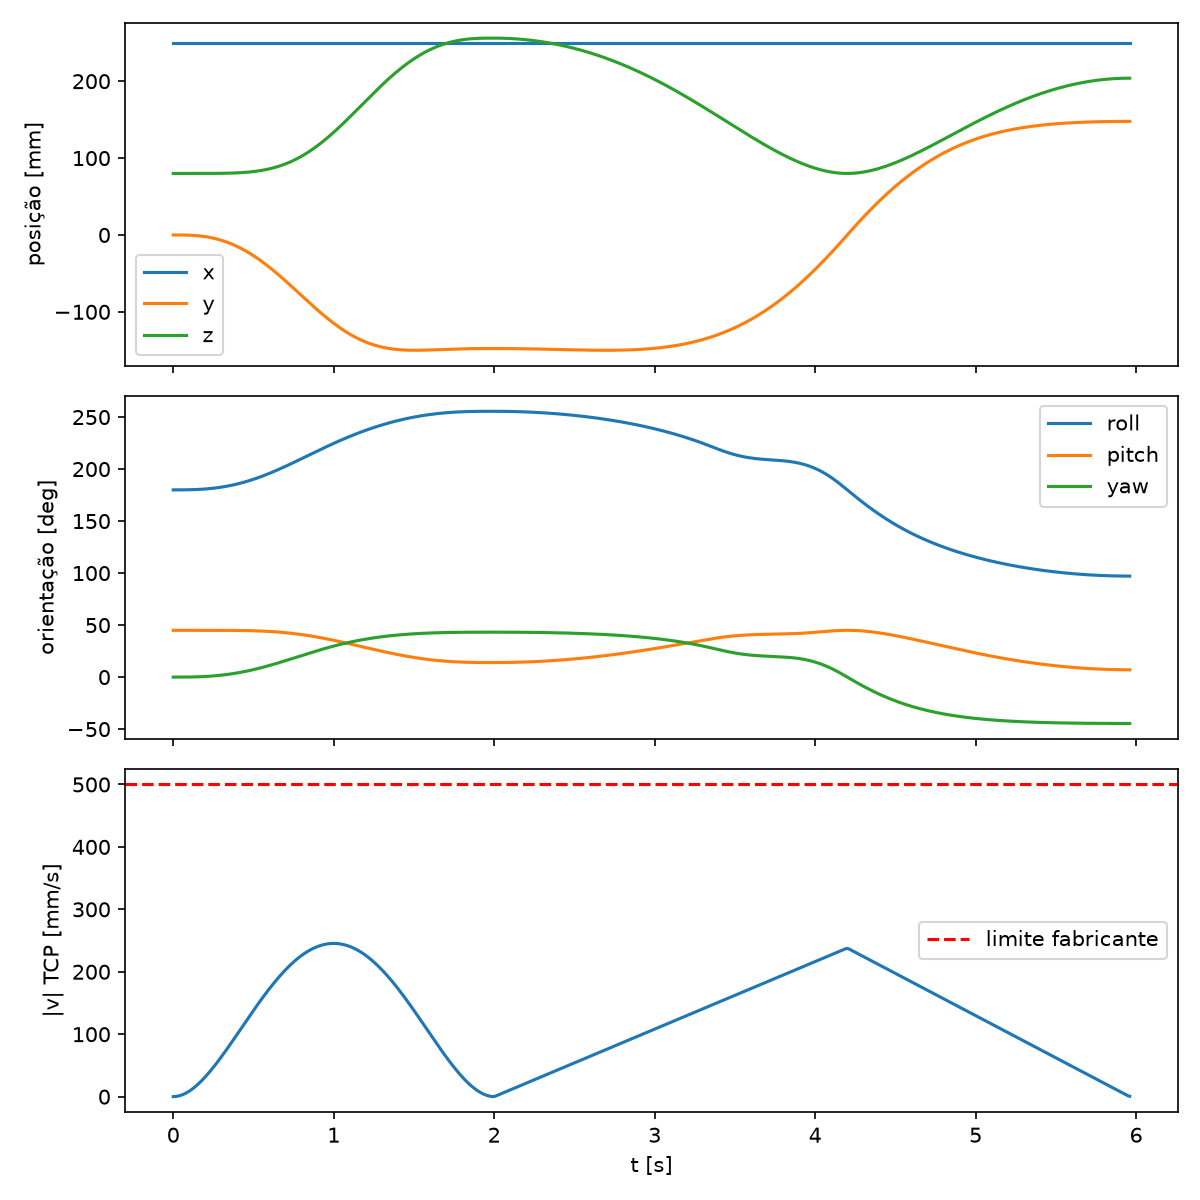
\includegraphics[width=\linewidth]{traj_cartesiana.png}
% 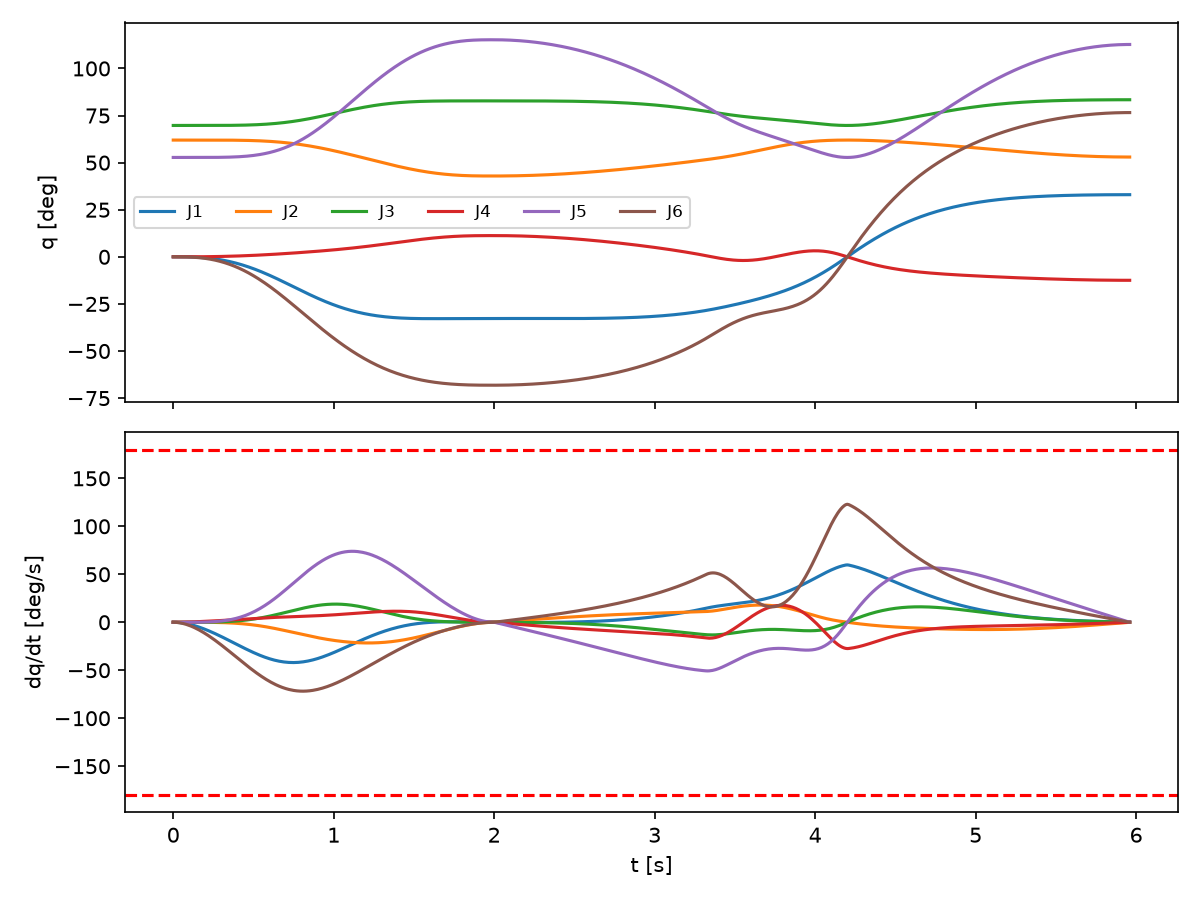
\includegraphics[width=\linewidth]{traj_juntas.png}
% 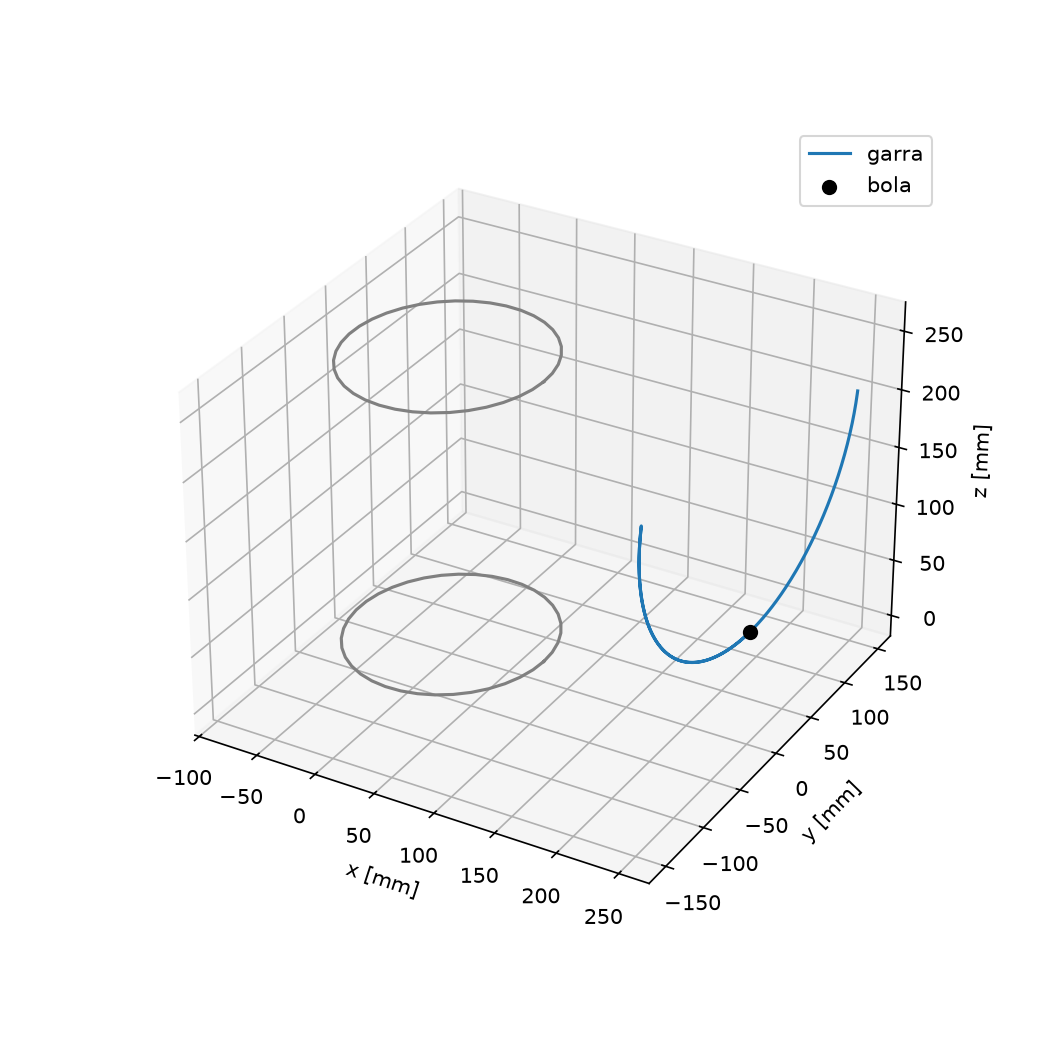
\includegraphics[width=.7\linewidth]{traj_3d.png}

\section{Tarefa 3 --- Execução no robô}
% Método (set_position com blending vs set_servo_cartesian), fator de
% abrandamento, referência vs pose medida (data/run_servo.csv).

\section{Tarefa 4 --- Precisão da cinemática inversa}
% IK do controlador -> FK própria; erros de posição/orientação ao longo da
% trajetória.
% 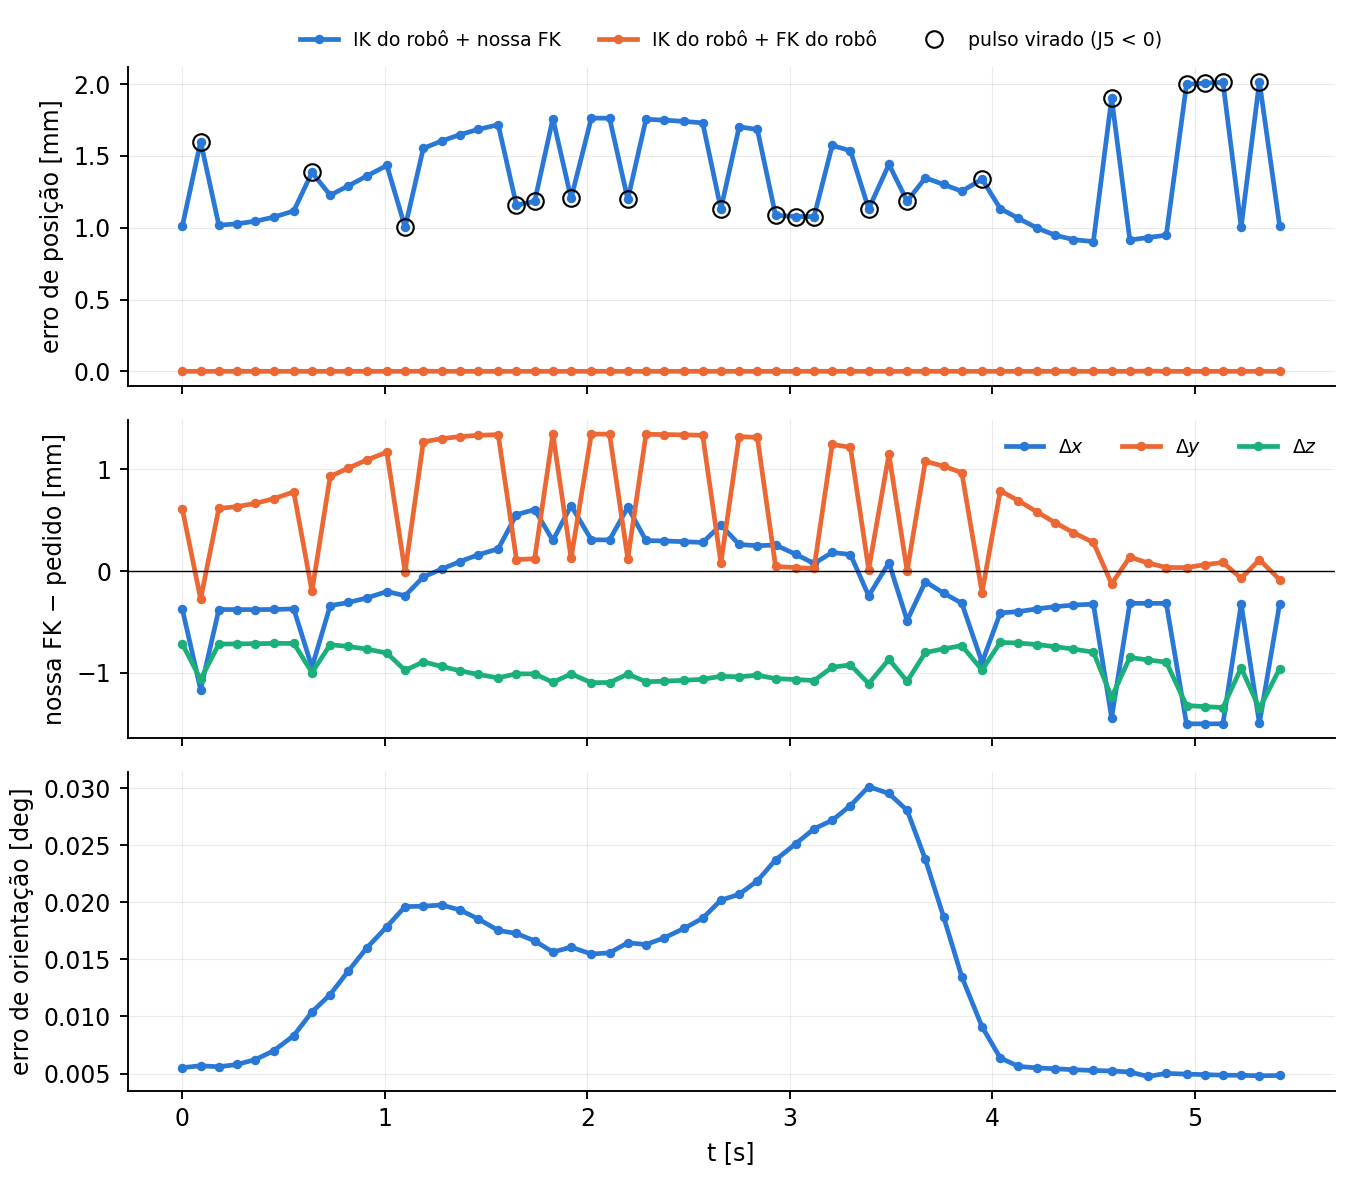
\includegraphics[width=\linewidth]{ik_erros.png}

\section{Conclusões}

\end{document}
